%%%%%%%%%%%%%%%%%%%%%%%%%%%%%%%%%%%%%%%%%%%%%%%%%%%%%%%
% Copyright (c) 2024 Fengming Zhu. All rights reserved.
% Email:        fzhuae@connect.ust.hk
%%%%%%%%%%%%%%%%%%%%%%%%%%%%%%%%%%%%%%%%%%%%%%%%%%%%%%%


\documentclass{beamer}
\usepackage{hyperref}
\usepackage[T1]{fontenc}
\usepackage[numbers]{natbib}
%\UseRawInputEncoding

\usetheme{metropolis}
\definecolor{white}{rgb}{1,1,1}
\beamersetaveragebackground{white}

% other packages
\usepackage{latexsym,amsmath,xcolor,multicol,booktabs,calligra}
\usepackage{amsfonts, amssymb}
\usepackage{graphicx,listings,stackengine}
\usepackage{ulem}

% \usepackage[loadonly]{enumitem}
% \setlistdepth{20}
% \renewlist{itemize}{itemize}{20}

%% Enable only in Xelatex
% \usepackage{pstricks}

\author{Fengming ZHU}  % you can change it to your name
\title{COMP3211 Tutorial 6: Markov Decision Process}
\institute{Department of CSE \\ HKUST \\ {\copyright\ 2024 Fengming Zhu. All rights reserved.}}
\date{\today} % you can change it to the latest date


% defs
\def\cmd#1{\texttt{\color{red}\footnotesize $\backslash$#1}}
\def\env#1{\texttt{\color{blue}\footnotesize #1}}
\definecolor{deepblue}{rgb}{0,0,0.5}
\definecolor{deepred}{rgb}{0.6,0,0}
\definecolor{deepgreen}{rgb}{0,0.5,0}
\definecolor{halfgray}{gray}{0.55}

\lstset{
    basicstyle=\ttfamily\small,
    keywordstyle=\bfseries\color{deepblue},
    emphstyle=\ttfamily\color{deepred},    % Custom highlighting style
    stringstyle=\color{deepgreen},
    numbers=left,
    numberstyle=\small\color{halfgray},
    rulesepcolor=\color{red!20!green!20!blue!20},
    frame=shadowbox,
}

{}
\begin{document}

\begin{frame}
    \titlepage
\end{frame}


% \begin{frame}{References}
% \begin{itemize}
%     \item \underline{Main focus}
%     \begin{itemize}
%         \item
%         (SoCS'2013) \textbf{Multi-Agent Path Finding for Self Interested Agents}
%         \cite{bnaya2013multi}
        
%         \item
%         (AAAI'2015) \textbf{Multi-Agent Pathfinding as a Combinatorial Auction}
%         \cite{amir2015multi}

%         \item
%         (Tech report) \textbf{An Empirical Evaluation of a Combinatorial Auction for Solving Multi-Agent Pathfinding Problems}
%     \end{itemize}

%     \item Related
%     \begin{itemize}
%         \item
%         (AAMAS'2019) \textit{Polynomial-Time Multi-Agent Pathfinding with Heterogeneous and Self-Interested Agents}
%         \cite{machida2019polynomial}

%         \item
%         (IROS'2020) \textit{Path Negotiation for Self-interested Multirobot Vehicles in Shared Space}
%         \cite{inotsume2020path}
%     \end{itemize}
% \end{itemize}
% \end{frame}


\begin{frame}{Outline}
    % \tableofcontents[sectionstyle=show,subsectionstyle=show/shaded/hide,subsubsectionstyle=show/shaded/hide]
    \tableofcontents[
    sectionstyle=show,
    subsectionstyle=shaded,
    subsubsectionstyle=shaded
    ]
\end{frame}


\section{MDP V.S. Search}


\begin{frame}{MDP V.S. Search}
    \begin{exampleblock}{Search:}
        \begin{itemize}
            \item A set of states $\mathcal{S}$, initial state $I$, goal state $G$

            \item A set of actions $\mathcal{A}$

            \item Deterministic transitions $T: \mathcal{S} \times \mathcal{A} \rightarrow \mathcal{S}$

            \item cost function $c: \mathcal{S} \times \mathcal{A} \rightarrow \mathbb{R}$

            \item Objective: a path $p$ from $I$ to $G$ that minimizes $c(p)$
        \end{itemize}
    \end{exampleblock}

    \pause
    \begin{exampleblock}{MDP:}
        \begin{itemize}
            \item A set of states $\mathcal{S}$, a terminating condition $End(s)$

            \item A set of actions $\mathcal{A}$

            \item Stochastic transitions $T: \mathcal{S} \times \mathcal{A} \rightarrow \Delta(\mathcal{S})$

            \item Reward function $r: \mathcal{S} \times \mathcal{A} \rightarrow \mathbb{R}$, with a discount factor $\gamma$

            \item Objective: maximize $\sum_t \gamma^t r_t$
        \end{itemize}
    \end{exampleblock}
\end{frame}

\begin{frame}{Solution Concept: Policy}
    \begin{exampleblock}{Question:}
        To make sure you can come up with an optimal solution, you'd like to know:
        \begin{itemize}
            \item (A) Only your current state

            \item (B) All the history from the beginning up until now

            \item (C) Need to know more
        \end{itemize}
    \end{exampleblock}

    \pause
    \begin{exampleblock}{Markov property:}
        A state $S_t$ is Markovian iff $P[S_{t+1}| S_{t}, \cdots, S_0] = P[S_{t+1}| S_{t}]$.
        That is, your current state is already a ``sufficient statistic'',
        also known as the \alert{information state}.
    \end{exampleblock}

    \pause
    \begin{exampleblock}{Policy:}
        A solution is a policy $\pi: \mathcal{S} \rightarrow \Delta(\mathcal{A})$ 
    \end{exampleblock}

\end{frame}

\begin{frame}{Follow-up Question: Maze}
    \begin{exampleblock}{Question:}
        Given a large maze,
        you (with deterministic actions U/D/L/R) are supposed to find a nice way from the entrance to the exit,
        which agent you'd like to choose
        \begin{itemize}
            \item (A) State machines with infite memory
            \item (B) Agents that can $A^*$ search
            \item (C) Agents that can compute policies
            \item (D) None of them
        \end{itemize}
        
        \begin{figure}[htpb]
            \centering
            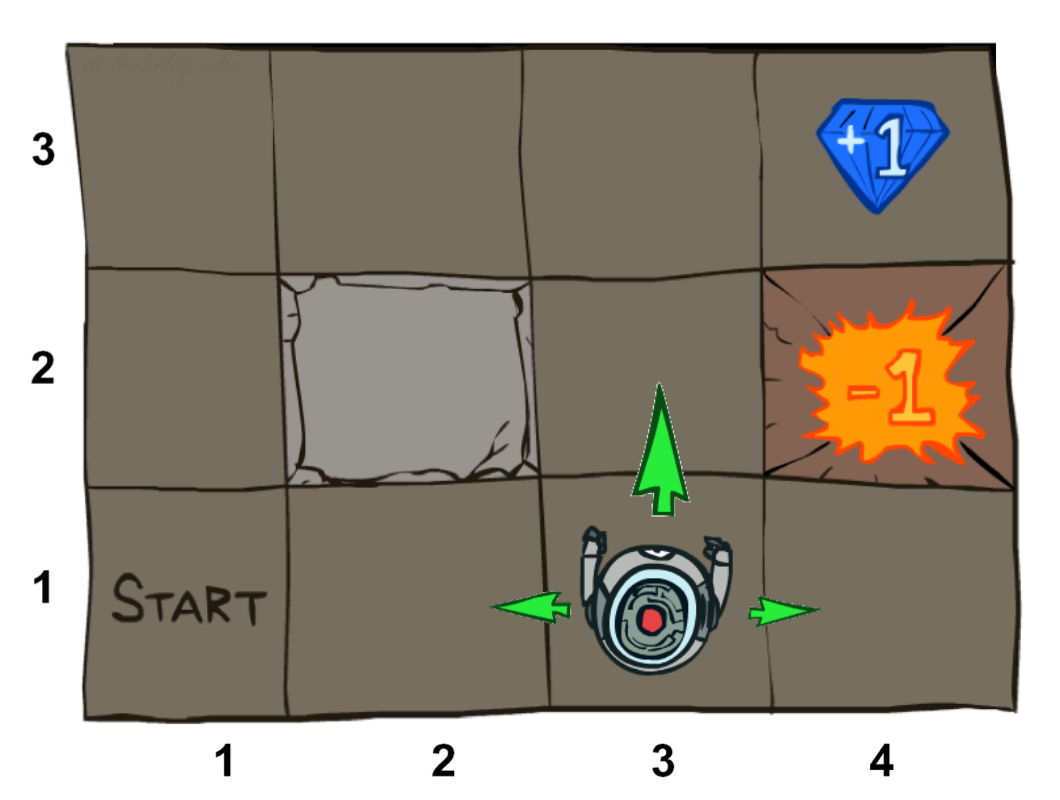
\includegraphics[width=0.3\linewidth]{pic/maze.png}
            \pause
            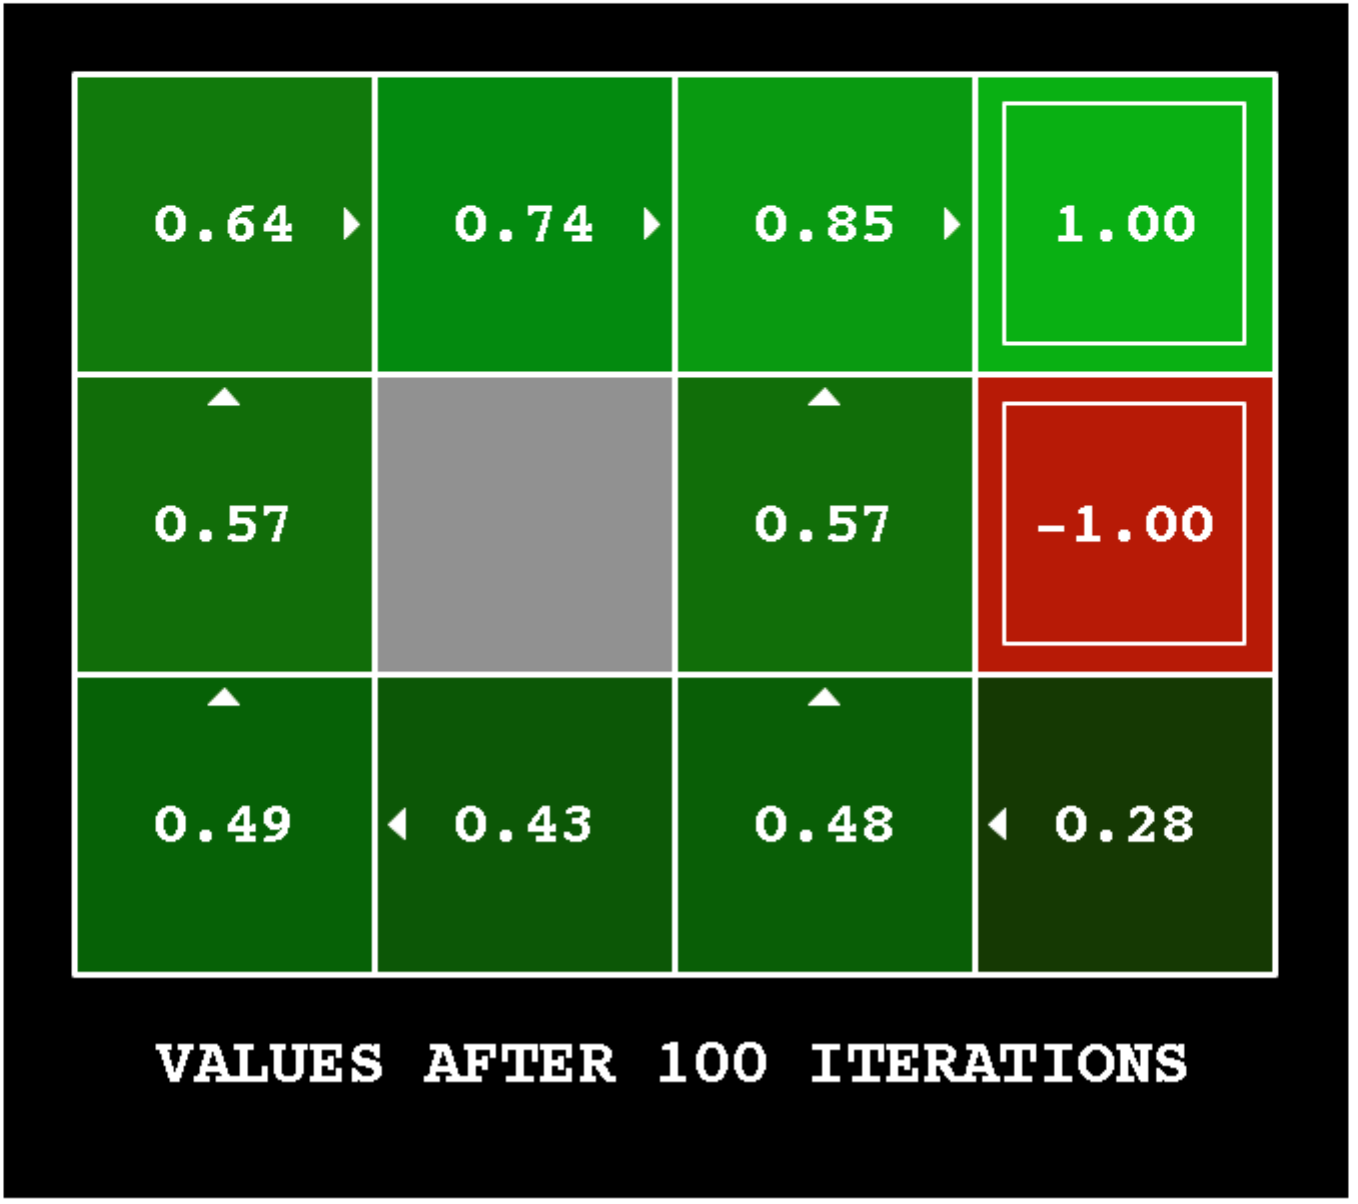
\includegraphics[width=0.25\linewidth]{pic/maze_ret.png}
        \end{figure}
    \end{exampleblock}
\end{frame}


\section{Value Functions}

% TODO
\begin{frame}{Notations with Time Index}

\begin{itemize}
    \item \alert{Transition:}
    $T_{s,s'}^a = \mathbb{P}[S_{t+1}=s'|S_t=s, A_t=a]$
    \item \alert{Reward:}
    $R_{s}^a = \mathbb{E}[R_{t+1}|S_t=s, A_t=a]$
    \item \alert{Stationary policy:}
    $\pi(a|s) = \mathbb{P}[A_t = a | S_t=s]$
    \item \alert{Return:}
    The return $G_t$ is the total discounted reward from time $t$,
    \[
    G_t = R_{t+1} + \gamma R_{t+2} + \cdots
        = \sum_{k=0}^\infty \gamma^k R_{t+k+1}
    \]
\end{itemize}

\end{frame}


\begin{frame}{$v(s)$ and $q(s,a)$}
% problem := solve G, V, Q, \pi!
\begin{exampleblock}{State-value function:}
    The state-value function $v_\pi(s)$ for an MDP is the expected
    return starting from state s, and then following policy $\pi$,
    \[
        v_\pi(s) = \mathbb{E}_\pi[G_t|S_t = s]
    \]
\end{exampleblock}

\begin{exampleblock}{Action-value function:}
    The action-value function $q_\pi(s,a)$ for an MDP is the expected
    return starting from state s, taking action a,
    and then following policy $\pi$,
    \[
        q_\pi(s,a) = \mathbb{E}_\pi[G_t|S_t = s, A_t = a]
    \]
\end{exampleblock}   
\end{frame}


\begin{frame}{Policy Interation}
    \begin{exampleblock}{Policy iteration:}
  	\begin{itemize}
  		\item Initialize $\pi \gets \pi_0$
  		\item While $\pi$ still changing:
  		\begin{itemize}
  			\item \underline{Policy evaluation}: iterate until convergence
  			$\forall s,
  			v^t_\pi(s) = \sum_{s'\in S} T(s, \pi(s), s')[R(s, \pi(a), s') + \gamma v^{t-1}_\pi(s')]$
  			\item \underline{Policy improvement}: greedy update
			$\forall s,
			\pi_{new}(s) = \arg\max_{a\in A(s)} q_{\pi}(s, a)$
  			\item $\pi \gets \pi_{new}$
  		\end{itemize}
  	\end{itemize}
    \end{exampleblock}
\end{frame}


\section{Bellman Expectation Equation}



\begin{frame}{Bellman Expectation Equation}
    \begin{itemize}
    	\item For \underline{policy evaluation}, we desire
  		\[
  		v_\pi(s) = \sum_{s'\in S} T(s, \pi(s), s')[R(s, \pi(a), s') + \gamma v_\pi(s')]
  		\]
        \item For state-value function,
        \[
        v_\pi(s) 
        = E_{\pi}[R_{t+1} + \gamma v_\pi(S_{t+1})|S_t = s]
        \]
        
        \item For action-value function,
        \[
        q_{\pi}(s, a) 
        = E_{\pi}[R_{t+1} 
        + \gamma q_{\pi}(S_{t+1}, A_{t+1})|S_t = s, A_t=a]
        \]
    \end{itemize}
\end{frame}

\begin{frame}{Bellman Expectation Equation}

\end{frame}

\begin{frame}{Warming-up: Adam's Law}
    \begin{exampleblock}{Adam's Law:}
        For any random variables $X$ and $Y$,
        \[
        {E}[ {E}[ X|Y ] ] = {E}[ X ]
        \]
    \end{exampleblock}

    \begin{exampleblock}{Adam's Law with Extra Conditioning:}
        For any random variables $X$, $Y$ and $Z$,
        \[
        {E}[ {E}[ X|Y,Z ]|Z ] = {E}[ X|Z ]
        \]
    \end{exampleblock}
\end{frame}

\begin{frame}{Bellman Expectation Equation for $v^\pi(s)$}
    We first prove the Bellman equation for state-value function.
    \[
    \begin{split}
    v_{\pi}(S_t=s) 
        & = E_{\pi}[G_t|S_t = s]\\
        & = E_{\pi}[R_{t+1} 
        + \gamma (R_{t+2} + \gamma R_{t+3} +\cdots) |S_t = s]\\
        & = E_{\pi}[R_{t+1} + \gamma G_{t+1}|S_t = s] \\
    \end{split}
    \]
    Since
    \[
    \begin{split}
        E_{\pi}[G_{t+1}|S_t] & = E_{\pi}[E_{\pi}[G_{t+1}|S_{t+1}, S_t]|S_t] \\
        & = E_{\pi}[E_{\pi}[G_{t+1}|S_{t+1}]|S_t] \\
        & = E_{\pi}[v_\pi(S_{t+1})|S_t]
    \end{split}
    \]
    Thus,
    \[
    \begin{split}
        v(S_t = s) &= E_{\pi}[G_t|S_t = s] \\
        & = E_{\pi}[R_{t+1} + \gamma G_{t+1}|S_t = s] \\
        & = E_{\pi}[R_{t+1} + \gamma v_\pi(S_{t+1})|S_t = s]
    \end{split}
    \]
\end{frame}


\begin{frame}{Bellman Expectation Equation for $q^\pi(s,a)$}
    We then prove the Bellman equation for action-state function. 
    \[
    \begin{split}
    q_{\pi}(S_t=s, A_t=a) 
    & = E_{\pi}[G_t |S_t = s, A_t=a] \\
    & = E_{\pi}[R_{t+1} + \gamma G_{t+1}|S_t = s, A_t=a]
    \end{split}
    \]
    Since
    \[
    \begin{split}
        E[G_{t+1}|S_t, A_t] 
        &= E[E[G_{t+1}|(S_{t+1}, A_{t+1}),(S_t, A_t)]|(S_t, A_t)] \\
        &= E[E[G_{t+1}|(S_{t+1}, A_{t+1})]|(S_t, A_t)] \\ 
    \end{split}
    \]
    Under policy $\pi$, we have
    \[
    \begin{split}
        E_{\pi}[G_{t+1}|S_t, A_t] 
        & = E_{\pi}[E_{\pi}[G_{t+1}|(S_{t+1}, A_{t+1})]|(S_t, A_t)] \\
        & = E_{\pi}[q_{\pi}(S_{t+1}, A_{t+1})|(S_t, A_t)] \\
    \end{split}
    \]
    Thus,
    \[
    \begin{split}
    q_{\pi}(S_t=s, A_t=a) 
    & = E_{\pi}[R_{t+1} + \gamma G_{t+1}|S_t = s, A_t=a] \\
    & = E_{\pi}[R_{t+1} + \gamma q_{\pi}(S_{t+1}, A_{t+1})|S_t = s, A_t=a] \\
    \end{split}
    \]

\end{frame}

\section{Bellman Optimality Equation}

\begin{frame}{Optimal Value Function}
    \begin{itemize}
        \item For state-value function,
        \[
        v_*(s) 
        = \max_{\pi} v_\pi (s)
        \]
        
        \item For action-value function,
        \[
        q_*(s, a) 
        = \max_\pi q_\pi(s, a) 
        \]

        \item The optimal value function specifies the best possible
        performance in the MDP.

        \item An MDP is ``solved'' once we know the optimal values.
    \end{itemize}
\end{frame}


\begin{frame}{Optimal Policy}
    \begin{exampleblock}{Define a partial ordering over policies:}
        $$
        \pi \geq \pi' \text{, if } v_\pi(s) \geq v_\pi'(s)
        \text{, for all } s.
        $$
    \end{exampleblock}

    \pause
    \begin{exampleblock}{For any MDP:}
        \begin{itemize}
            \item There exists an optimal policy $\pi_*$ that is better than or
            equal to all other policies,
            $\pi_* \geq \pi$, for all $\pi$.
            
            \item All optimal policies achieve the optimal state-value function, 
            $v_{\pi_*}(s) = v_*(s)$, for all $s$.

            \item All optimal policies achieve the optimal action-value function,
            $q_{\pi_*}(s,a) = q_*(s,a)$, for all $s, a$.
        \end{itemize}
    \end{exampleblock}
\end{frame}


\begin{frame}{Finding Optimal Policy}
\begin{exampleblock}{Theorem:}
    \begin{itemize}
        \item An optmial policy can be found by maximizing over $q_*(s,a)$,
        \[
        \pi_*(a|s) = 
        \begin{cases}
            1 & \text{, if } a = argmax_{a\in A} q_*(s, a)\\
            0 & \text{, otherwise}\\
        \end{cases}
        \]

        \item There is always a \alert{deterministic} optimal policy for any MDP.

        \item If we know $q_*(s,a)$, we immediately have the optimal policy.
    \end{itemize}
\end{exampleblock}
\end{frame}


\begin{frame}{Bellman Optimality Equation}
    \begin{itemize}
        \item For state-value function,
        \[
        v_*(s) = \max_a E[R_{t+1} + \gamma v_*(S_{t+1})|S_t=s, A_t=a]
        \]
        
        \item For action-value function,
        \[
        q_*(s,a) 
        = E[R_{t+1} + \gamma \max_{a'}q_*(S_{t+1}, a') |S_t=s, A_t=a]
        \]
        \item \alert{However,} non-linear thus no closed form solution in general.
    \end{itemize}
\end{frame}


% TODO 
\begin{frame}{Bellman Optimality Equation for $v_*$ and $q_*$}
    Under the optimal policy, we first show the relation of $v^*$ and $q^*$.
    \begin{itemize}
        \item $v_*$ in terms of $q_*$,
        \[
        v_*(s) = \max_a q_*(s,a)
        \]
        
    \end{itemize}
\end{frame}

\begin{frame}{Bellman Optimality Equation for $v_*$ and $q_*$ (cont'd)}
    \begin{itemize}
        \item $q_*$ in terms of $v_*$,
        \[
        \begin{split}
             q_*(s,a) &= \max_\pi q_\pi(s,a) \\
             & = R_s^a + \gamma \sum_{s'}T^a_{ss'} \max_\pi v_\pi(s') \\
             & = R_s^a + \gamma \sum_{s'}T^a_{ss'}v_*(s') \\
             & = E[R_{t+1}|S_t=s, A_t=a] \\
             & + \gamma \sum_{s'} \{ P(S_{t+1}=s'|S_t=s, A_t=a) \\
             & \cdot E[v_*(S_{t+1})|S_{t+1}=s', S_t=s, A_t=a] \} \\
             & = E[R_{t+1}|S_t=s, A_t=a] + \gamma E[v_*(S_{t+1})|S_t=s, A_t=a] \\
             & = E[R_{t+1} + \gamma v_*(S_{t+1})|S_t=s, A_t=a]
        \end{split}
        \]  
    \end{itemize}
\end{frame}

\begin{frame}{Bellman Optimality Equation for $V_*$ and $Q_*$}
    Then we show the Bellman optimal equation for $v^*$,
    \[
    \begin{split}
        v_*(s) &= \max_a q_*(s,a) \\
        & = \max_a E[R_{t+1} + \gamma v_*(S_{t+1})|S_t=s, A_t=a]
    \end{split}
    \]
    Finally, we show the Bellman equation for $q^*$,
    \[
    \begin{split}
        q_*(s,a) 
        &= E[R_{t+1} + \gamma v_*(S_{t+1})|S_t=s, A_t=a] \\
        &= E[R_{t+1} + \gamma \max_{a'}q_*(S_{t+1}, a') |S_t=s, A_t=a]
    \end{split}
\]
\end{frame}


\begin{frame}{One Last Remark on PI v.s. VI}

\end{frame}


% \begin{frame}{Cooperative v.s. Self-interested}

% \begin{exampleblock}{Cooperative agents:}
% \begin{itemize}
%     \item Input: {a weighted graph, N agents (starts/goals)}
    
%     \item Objective: {minimize global cost}
% \end{itemize}
% \end{exampleblock}

% \pause
% \begin{exampleblock}{Self-interested agents:}
% \begin{itemize}
%     \item Objective: {minimize \textbf{individual cost}}

%     \pause
%     \item A naïve way: {each schedule herself individually, resolve conflicts randomly}
% \end{itemize}
% \end{exampleblock}

% \end{frame}


% \begin{frame}{Relation with Traffic Control}

% \begin{exampleblock}{Traffic flow network:}
% \begin{itemize}
%     \item Continuous flow along edges, causing certain \alert{delays}

%     \item Selfish routing is proved to be non-optimal

%     \item Toll/taxation mechanisms are usaully used.

%     \item Sometimes coincides with congestion games (a classical \alert{potential game}) 
% \end{itemize}
% \end{exampleblock}

% \end{frame}



% \begin{frame}{An Example}

% % \begin{figure}[htpb]
% %         \centering
% %         \includegraphics[width=0.6\linewidth]{pic/tax_eg.png}
% % \end{figure}

% \begin{columns}
%     \begin{column}{.5\textwidth}
%     \centering
%         \underline{Selfish routing} \\
%         a1: \{S1, \_, C, G1\} \\
%         a2: \{S2, C, G2\} \\
%         a3: \{S3, \_, C, G3\} \\
%         $\Rightarrow (3+\alert{1}) + 2 + (3+\alert{2}) = 11$
%     \end{column}    

%     \pause
%     \begin{column}{.5\textwidth}
%     \centering
%         \underline{With taxation} \\
%         a1: \{S1, left-hand, G1\} \\
%         a2: \{S2, C, G2\} \\
%         a3: \{S3, right-hand, G3\} \\
%         $\Rightarrow \alert{4} + 2 + \alert{4} = 10$
%     \end{column}
% \end{columns}

% \end{frame}


% \begin{frame}{Formally}

% \begin{exampleblock}{Key idea:}
% \begin{itemize}
%     \item Assign each edge/vertex a tax (penalty)

%     \item Individually minimizes $\hat{c}(P_i) = c(P_i) + T(P_i)$

%     \pause[2]
%     \item \alert{$\Rightarrow$ Iterative Taxation Framework}
%     % \begin{figure}[htpb]
%     %     \centering
%     %     \includegraphics[width=0.8\linewidth]{pic/ITF.png}
%     % \end{figure}

%     \pause[3]
%     \item Implementations: 1) Exhaustive 2) Monte-Carlo
% \end{itemize}
% \end{exampleblock}

% \end{frame}


% \begin{frame}{Evaluation -- toy example}

% % \begin{figure}[htpb]
% %         \centering
% %         \includegraphics[width=1\linewidth]{pic/result_3x3.png}
% %         \caption{EITA (exhaustive iterative taxation algorithm),
% %                 MC-ITA (Monte-Carlo iterative taxation algorithm),
% %                 Lowerbound (global optimum)} 
% % \end{figure}

% \end{frame}


% \begin{frame}{Evaluation -- large scale}

% \begin{columns}
%     \begin{column}{.65\columnwidth}
%         % \begin{figure}[htpb]
%         %     \centering
%         %     \includegraphics[width=1\linewidth]{pic/result_den520.png}
%         %     \caption{den520d for 10 agents}
%         % \end{figure}
%     \end{column}

%     \begin{column}{.35\columnwidth}
%         % \begin{figure}[htpb]
%         %     \centering
%         %     \includegraphics[width=1\linewidth]{pic/den520d.pdf}
%         %     \caption{den520d -- dimension ($257\times 256$), \#states (28178)}
%         % \end{figure}
%     \end{column}
% \end{columns}

% \end{frame}


% \begin{frame}{Drawbacks}

% \begin{itemize}
%     \item Not guaranteed to minimize global cost (maximize social welfare)

%     \item Not strategyproof: agents could misreport their starts/goals

%     \item Agents are restricted to be homogeneous

%     \pause
%     \item \alert{Let's seek help from auctions!}
% \end{itemize}

% \end{frame}



% \begin{frame}{Conventional Combinatorial Auction}

% \begin{exampleblock}{Preliminaries}
%     \begin{itemize}
%         \item Agents: $N = \{1, \cdots, n\}$

%         \item Actioned items: $M = \{1, \cdots, m\}$

%         \item Valuation function for each agent $v_i: 2^M \mapsto \mathbb{R}$

%         \pause
%         \alert{
%         \item A mechanism (with monetary transfer) is a pair of
%         \begin{itemize}
%             \item a social choice function $f: V_1 \times \cdots \times V_n \mapsto A$
            
%             \item a vector of payments functions $p_1, \cdots, p_n$, where $p_i: V_1 \times \cdots \times V_n \mapsto \mathbb{R}$
%         \end{itemize}}
%     \end{itemize}
% \end{exampleblock}

% \end{frame}


% \begin{frame}{Reduce to CA}

%     % \begin{figure}[htpb]
%     %     \centering
%     %     \includegraphics[width=1\linewidth]{pic/reduction.png}
%     % \end{figure}

%     \pause
%     \begin{exampleblock}{Derived valuation function:}
%     \begin{itemize}[<+-| alert@+>]
%         \item $v_i(p) = val(g_i) - c(p)$

%         \item Turns out $val(g_i) := max_c \times n$ [constant]
%     \end{itemize}
%     \end{exampleblock}

% \end{frame}


% \begin{frame}{Strategic Manipulation}

%     % \begin{figure}[htpb]
%     %     \centering
%     %     \includegraphics[width=0.4\linewidth]{pic/ca_eg.png}
%     %     \caption{Assuming $v_i(g_i) = 10$}
%     % \end{figure}

%     \begin{exampleblock}{A centralized yet not strategyproof mechanism:}
%     \begin{itemize}[<+-| alert@+>]
%         \item If a1 and a2 report truthfully,
%             \begin{itemize}
%                 \item a1 gets 10-(1.5+1), a2 gets 10-(1+1)
%             \end{itemize}

%         \item If a1 misreports (s1, X) = 1.8,
%             \begin{itemize}
%                 \item a1 gets 10-(1+1), a2 gets 10-(1.7+1)
%             \end{itemize}
%     \end{itemize}
%     \end{exampleblock}

% \end{frame}


% \begin{frame}{Strategic Manipulation}

%     % \begin{figure}[htpb]
%     %     \centering
%     %     \includegraphics[width=0.3\linewidth]{pic/ca_eg.png}
%     %     \caption{Assuming $v_i(g_i) = 10$}
%     % \end{figure}

%     \begin{exampleblock}{The well-known VCG mechanism:}
%     \begin{itemize}[<+-| alert@+>]
%         \item Payment := the harm you did to others' social welfare

%         \item If a1 and a2 report truthfully,
%             \begin{itemize}
%                 \item a1 gets 10-(1.5+1)-0 = 7.5, a2 gets 10-(1+1)-0.5
%             \end{itemize}

%         \item If a1 misreports (s1, X) = 1.8,
%             \begin{itemize}
%                 \item a1 gets 10-(1+1)-0.7 = 7.3, a2 gets 10-(1.7+1)-0
%             \end{itemize}
%     \end{itemize}
%     \end{exampleblock}

% \end{frame}


% \begin{frame}{Computational Issues}

% \begin{itemize}
%     \item In sealed-bid auctions, such as VCG, each agent needs to bid over all bundles that it may be interested in. 

%     \item In MAPF, this means that an agent $i$ would need to find all paths from $s_i$ to $g_i$ and place bids on them.

%     \item The number of paths between two vertices in a graph may be exponential in the path length.

%     \item Moreover, to find an allocation that maximizes its revenue, the auctioneer will need to check the cross product of these potentially exponential number of bids.

%     \pause
%     \item \alert{Interative combinatorial auction (Parkes 2006)}
% \end{itemize}

% \end{frame}


% \begin{frame}{Iterative Combinatorial Auction}

% \begin{exampleblock}{Basic framework (\textit{iBundle}):}
% \begin{itemize}
%     \item Bidding

%     \item Winner determination

%     \item Price update
% \end{itemize}
% \end{exampleblock}

% \end{frame}


% \begin{frame}{iBundle -- Bidding}

%     % \begin{figure}[htpb]
%     %     \centering
%     %     \includegraphics[width=0.8\linewidth]{pic/bidding.png}
%     % \end{figure}

%     \begin{exampleblock}{Bidding:}
%         \begin{itemize}[<+-| alert@+>]
%             \item Agents place \texttt{XOR} bids on their \underline{desired} bundles.

%             \item Minimize $cost(p) + ask(p)$

%             \item $a_3$ bids $[<F, t_1>, <D, t_2>, <G, t_3>, <E, t_4>, <I, t_5>]; [<F, t_1>, <D, t_2>, <C, t_3>, <E, t_4>, <I, t_5>]$.

%             \item Myopic best response is a dominant strategy
%         \end{itemize}
%     \end{exampleblock}

% \end{frame}


% \begin{frame}{iBundle -- Winner Dermination}

%     % \begin{figure}[htpb]
%     %     \centering
%     %     \includegraphics[width=0.8\linewidth]{pic/bidding.png}
%     % \end{figure}

%     \begin{exampleblock}{Winner determination:}
%         \begin{itemize}[<+-| alert@+>]
%             \item Determine a provisional allocation

%             \item To maximizes seller's revenue and include more non-conflicting agents

%             \item $a_1$ gets $[<A, t_1>, <C, t_2>]$, $a_3$ gets $[<F, t_1>, <D, t_2>, <G, t_3>, <E, t_4>, <I, t_5>]$
%         \end{itemize}
%     \end{exampleblock}

% \end{frame}


% \begin{frame}{iBundle -- Price Update}

%     % \begin{figure}[htpb]
%     %     \centering
%     %     \includegraphics[width=0.8\linewidth]{pic/bidding.png}
%     % \end{figure}

%     \begin{exampleblock}{Price update:}
%         \begin{itemize}[<+-| alert@+>]
%             \item Initial prices for all bundles are 0

%             \item Bundles that ``unhappy'' agents bid on are raised by $\epsilon$

%             \item In MAPF, sufficient to set $\epsilon = \min(c_e)$

%             \item $a_2$ is unhappy, prices of paths of $MDD_2^3$ are raised by 1
%         \end{itemize}
%     \end{exampleblock}

% \end{frame}


% \begin{frame}{Evaluation}
%     % \begin{figure}[htpb]
%     %     \includegraphics[width=0.6\linewidth]{pic/ca_small}
%     % \end{figure}
% \end{frame}


% \begin{frame}{Evaluation}
%     % \begin{figure}[htpb]
%     %     \includegraphics[width=0.6\linewidth]{pic/ca_large}
%     % \end{figure}
% \end{frame}



% %%%%%%%%%% part 4 %%%%%%%%%%


% \begin{frame}{Insights}

% \begin{itemize}[<+-| alert@+>]
%     \item Consider heterogeneous and self-interested agents

%     \item Still, complexity issues due to the combinatorial nature

%     \item One-parameter agents, e.g. fuel consumption  
%     \begin{itemize}
%         \item Seems poly-time strategyproof mechanism exists \cite{machida2019polynomial}
%     \end{itemize}

%     \item Negotiation and bargaining on paths\cite{inotsume2020path}
% \end{itemize}

% \end{frame}


% \begin{frame}[allowframebreaks]
%     \bibliography{ref}
%     \bibliographystyle{alpha}
%     % If too many references, use this command to resize:
%     % \tiny\bibliographystyle{alpha}
% \end{frame}


\begin{frame}
    \begin{center}
        {\Huge\calligra Thanks!}
    \end{center}
\end{frame}


% \begin{frame}{A Running Example}
    % \begin{figure}[htpb]
    %     \centering
    %     \includegraphics[width=0.5\linewidth]{pic/mapf_ca_eg.png}
        
    %     \pause
    %     \includegraphics[width=1\linewidth]{pic/mapf_ca_proc_1.png}
        
    %     \pause
    %     \includegraphics[width=1\linewidth]{pic/mapf_ca_proc_2.png}
        
    %     \pause
    %     \includegraphics[width=1\linewidth]{pic/mapf_ca_proc_3.png}
    % \end{figure}
% \end{frame}

% \begin{frame}{Sequential $\to$ Decentralized}
%     \begin{block}{}
%         \begin{figure}[htpb]
%             \centering
%             \includegraphics[width=0.3\linewidth]{pic/gradient.png}
%         \end{figure}
%     \end{block}

%     \pause
%     \begin{columns}
%         \begin{column}{.5\textwidth}
%         \centering
%             \begin{exampleblock}{Sequential update}
%                 \begin{itemize}
%                     \item
%                     For $i = 1 \to k$,
%                     \begin{itemize}
%                         \item While not converge,
%                         \begin{itemize}
%                             \item \texttt{Gradient ascent}
%                         \end{itemize}
%                     \end{itemize}
%                 \end{itemize}
%             \end{exampleblock}
%         \end{column}    

%         \pause
%         \begin{column}{.5\textwidth}
%         \centering
%             \begin{exampleblock}{Decentralized update}
%                 \begin{itemize}
%                     \item
%                     For every $i \in [1..k]$,
%                     \begin{itemize}
%                         \item While not converge,
%                         \begin{itemize}
%                             \item \texttt{Gradient ascent}
%                             \item \alert{\texttt{Broadcast}$({v}_i)$}
%                         \end{itemize}
%                     \end{itemize}
%                 \end{itemize}
%             \end{exampleblock}
%         \end{column}
%     \end{columns}
% \end{frame}


% \begin{frame}{Issues}
%     \begin{columns}
%         \begin{column}{.3\columnwidth}
%             \begin{figure}[htpb]
%                 \centering
%                 \includegraphics[width=1.1\linewidth]{pic/bias.png}
%             \end{figure}
%         \end{column}

%         \begin{column}{.7\columnwidth}
%             \begin{itemize}[<+-| alert@+>]
%                 \item 
%                 MNIST for minibatch sizes of 1024 (top), 512 (middle), and 256 (bottom)

%                 \item
%                 The figure shows the performance of EigenGame degrades in the low batch size regime.

%                 % \item
%                 % Because we use the same minibatch for all inner products in the gradient which contains products and ratios of random variables.

%                 \item Current hardware easily supports batches of 1024 for MNIST and 128 for IMAGENET

%                 \item \underline{\textbf{But still, can we reduce the bias?}}
%             \end{itemize}
%         \end{column}
%     \end{columns}
% \end{frame}


% \begin{frame}{Figure and Column}
%     % From thuthesis user guide.
%     \begin{minipage}[c]{0.3\linewidth}
%     %%% DO NOT USE PSTricks in pdflatex
% %         \psset{unit=0.8cm}
% %         \begin{pspicture}(-1.75,-3)(3.25,4)
% %             \psline[linewidth=0.25pt](0,0)(0,4)
% %             \rput[tl]{0}(0.2,2){$\vec e_z$}
% %             \rput[tr]{0}(-0.9,1.4){$\vec e$}
% %             \rput[tl]{0}(2.8,-1.1){$\vec C_{ptm{ext}}$}
% %             \rput[br]{0}(-0.3,2.1){$\theta$}
% %             \rput{25}(0,0){%
% %             \psframe[fillstyle=solid,fillcolor=lightgray,linewidth=.8pt](-0.1,-3.2)(0.1,0)}
% %             \rput{25}(0,0){%
% %             \psellipse[fillstyle=solid,fillcolor=yellow,linewidth=3pt](0,0)(1.5,0.5)}
% %             \rput{25}(0,0){%
% %             \psframe[fillstyle=solid,fillcolor=lightgray,linewidth=.8pt](-0.1,0)(0.1,3.2)}
% %             \rput{25}(0,0){\psline[linecolor=red,linewidth=1.5pt]{->}(0,0)(0.,2)}
% % %           \psRotation{0}(0,3.5){$\dot\phi$}
% % %           \psRotation{25}(-1.2,2.6){$\dot\psi$}
% %             \psline[linecolor=red,linewidth=1.25pt]{->}(0,0)(0,2)
% %             \psline[linecolor=red,linewidth=1.25pt]{->}(0,0)(3,-1)
% %             \psline[linecolor=red,linewidth=1.25pt]{->}(0,0)(2.85,-0.95)
% %             \psarc{->}{2.1}{90}{112.5}
% %             \rput[bl](.1,.01){C}
% %         \end{pspicture}
%     \end{minipage}\hspace{1cm}
%     \begin{minipage}{0.5\linewidth}
%         \medskip
%         %\hspace{2cm}
%         \begin{figure}[h]
%             \centering
%             \includegraphics[height=.4\textheight]{pic/dtmf.pdf}
%         \end{figure}
%     \end{minipage}
% \end{frame}

% \begin{frame}[fragile]{\LaTeX{} Commands}
%     \begin{exampleblock}{Commands}
%         \centering
%         \footnotesize
%         \begin{tabular}{llll}
%             \cmd{chapter} & \cmd{section} & \cmd{subsection} & \cmd{paragraph} \\
%             Chapter & Section & Subsection & Paragraph \\\hline
%             \cmd{centering} & \cmd{emph} & \cmd{verb} & \cmd{url} \\
%             Centre Align & Emphasis & Verbatim & Hyperlink \\\hline
%             \cmd{footnote} & \cmd{item} & \cmd{caption} & \cmd{includegraphics} \\
%             Foodnote & Item & Caption & FigP\&Pic \\\hline
%             \cmd{label} & \cmd{cite} & \cmd{ref} \\
%             Label & Citing & Referring\\\hline
%         \end{tabular}
%     \end{exampleblock}
%     \begin{exampleblock}{Environment Command}
%         \centering
%         \footnotesize
%         \begin{tabular}{lll}
%             \env{table} & \env{figure} & \env{equation}\\
%             Table & Figure & Equation \\\hline
%             \env{itemize} & \env{enumerate} & \env{description}\\
%             Bullets & Numbering & Description \\\hline
%         \end{tabular}
%     \end{exampleblock}
% \end{frame}

% \begin{frame}[fragile]{\LaTeX{} Environment Command Samples}
%     \begin{minipage}{0.5\linewidth}
% \begin{lstlisting}[language=TeX]
% \begin{itemize}
%   \item A \item B
%   \item C
%   \begin{itemize}
%     \item C-1
%   \end{itemize}
% \end{itemize}
% \end{lstlisting}
%     \end{minipage}\hspace{1cm}
%     \begin{minipage}{0.3\linewidth}
%         \begin{itemize}
%             \item A
%             \item B
%             \item C
%             \begin{itemize}
%                 \item C-1
%             \end{itemize}
%         \end{itemize}
%     \end{minipage}
%     \medskip
%     \pause
%     \begin{minipage}{0.5\linewidth}
% \begin{lstlisting}[language=TeX]
% \begin{enumerate}
%   \item Class 1 
%   \item Class 2
%   \item Class 2
%   \begin{itemize}
%     \item[n+e] Student 1
%   \end{itemize}
% \end{enumerate}
% \end{lstlisting}
%     \end{minipage}\hspace{1cm}
%     \begin{minipage}{0.3\linewidth}
%         \begin{enumerate}
%             \item Class 1
%             \item Class 2
%             \item Class 3
%             \begin{itemize}
%                 \item[n+e] Student 1
%             \end{itemize}
%         \end{enumerate}
%     \end{minipage}
% \end{frame}

% \begin{frame}[fragile]{\LaTeX{} Equations}
%     \begin{columns}
%         \begin{column}{.55\textwidth}
% \begin{lstlisting}[language=TeX]
% $V = \frac{4}{3}\pi r^3$

% \[
%   V = \frac{4}{3}\pi r^3
% \]

% \begin{equation}
%   \label{eq:vsphere}
%   V = \frac{4}{3}\pi r^3
% \end{equation}
% \end{lstlisting}
%         \end{column}
%         \begin{column}{.4\textwidth}
%             $V = \frac{4}{3}\pi r^3$
%             \[
%                 V = \frac{4}{3}\pi r^3
%             \]
%             \begin{equation}
%                 \label{eq:vsphere}
%                 V = \frac{4}{3}\pi r^3
%             \end{equation}
%         \end{column}
%     \end{columns}
%     \begin{itemize}
%         \item Check more \href{https://en.wikipedia.org/wiki/Help:Displaying_a_formula}{\color{purple}{Here}}
%     \end{itemize}
% \end{frame}

% \begin{frame}[fragile]
%     \begin{columns}
%         \column{.6\textwidth}
% \begin{lstlisting}[language=TeX]
% \begin{table}[htbp]
%   \caption{Definition}
%   \label{tab:number}
%   \centering
%   \begin{tabular}{cl}
%     \toprule
%     Word & Definition \\
%     \midrule
%     1 & 4.0 \\
%     2 & 3.7 \\
%     \bottomrule
%   \end{tabular}
% \end{table}
% Check definition of 
% Equation~(\ref{eq:vsphere}) 
% in Table~\ref{tab:number}。
% \end{lstlisting}
%         \column{.4\textwidth}
%         \begin{table}[htpb]
%             \centering
%             \caption{Definition}
%             \label{tab:number}
%             \begin{tabular}{cl}\toprule
%                 Eq. & Def. \\\midrule
%                 1 & 4.0\\
%                 2 & 3.7\\\bottomrule
%             \end{tabular}
%         \end{table}
%         \normalsize Please check the definition of Equation~(\ref{eq:vsphere}) in Table~\ref{tab:number}
%     \end{columns}
% \end{frame}

% \begin{frame}{Plotting}
%     \begin{itemize}
%         \item Vector: eps, ps, pdf
%         \begin{itemize}
%             \item METAPOST, pstricks, pgf $\ldots$
%             \item Xfig, Dia, Visio, Inkscape $\ldots$
%             \item Export Matlab / Excel as pdf
%         \end{itemize}
%         \item Bitmap: png, jpg, tiff $\ldots$
%         \begin{itemize}
%             \item Avoiding using bitmaps 
%         \end{itemize}
%     \end{itemize}
%     \begin{figure}[htpb]
%         \centering
%         \includegraphics[width=0.2\linewidth]{pic/QUT_Logo_CMYK.jpg}
%         \caption{This is a Bitmaps}
%     \end{figure}
% \end{frame}

\end{document}